\subsection{Predstavitev stroja in kosa}
Za svoj stroj sem si izbral dolgo-stružni avtomat Gauthier GM-127
prikazan na sliki \ref{gauthier_priblizano}.
Ima 5 držal za orodja in 3 gnana orodja, vidnih na spodnji
sliki \ref{gauthier_priblizano}. Omogoča struženje do ø12.7 mm.
Ima tudi možnost nadgradnje z roko za preprijem kosa pri odrezovanju in
povrtavanje ali vrezovanje navoja iz druge strani.

\begin{figure}[H]
	\begin{center}
		\includegraphics[width=8cm]{gauthier_slika.jpg}
		\caption{Slika stroja, katerega sem nastavljal
			\cite{interna}}
		\label{gauthier_priblizano}
	\end{center}
\end{figure}

Za izdelek, sem si izbral pušo iz materjala 1.4305.
Spodaj levo na sliki \ref{delavniska_risba} je delavniška risba z
merami in tolerancami kosa, desno pa je 3D model izdelka v izometričnem
pogledu, narejen v programu Blender.

\begin{figure}
	\begin{center}
		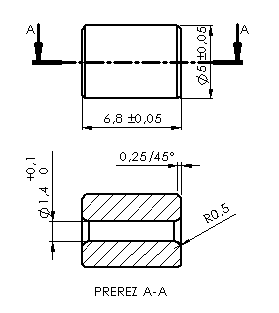
\includegraphics[width=8cm]{izdelek_risba.png}
		\caption{Risba končnika žice
			\cite{interna}}
		\label{delavniska_risba}
	\end{center}
\end{figure}

Izdelek se uporablja kot končnik žice, katera se napelje skozi
luknjo v sredini izdelka. Za lažjo napeljavo, so v luknji zahtevana
posnetja v obliki radiusa. Za tem se končnik fiksira z
stiskanjem v hidravlični stiskalnici.